\documentclass[1p]{elsarticle_modified}
%\bibliographystyle{elsarticle-num}

%\usepackage[colorlinks]{hyperref}
%\usepackage{abbrmath_seonhwa} %\Abb, \Ascr, \Acal ,\Abf, \Afrak
\usepackage{amsfonts}
\usepackage{amssymb}
\usepackage{amsmath}
\usepackage{amsthm}
\usepackage{scalefnt}
\usepackage{amsbsy}
\usepackage{kotex}
\usepackage{caption}
\usepackage{subfig}
\usepackage{color}
\usepackage{graphicx}
\usepackage{xcolor} %% white, black, red, green, blue, cyan, magenta, yellow
\usepackage{float}
\usepackage{setspace}
\usepackage{hyperref}

\usepackage{tikz}
\usetikzlibrary{arrows}

\usepackage{multirow}
\usepackage{array} % fixed length table
\usepackage{hhline}

%%%%%%%%%%%%%%%%%%%%%
\makeatletter
\renewcommand*\env@matrix[1][\arraystretch]{%
	\edef\arraystretch{#1}%
	\hskip -\arraycolsep
	\let\@ifnextchar\new@ifnextchar
	\array{*\c@MaxMatrixCols c}}
\makeatother %https://tex.stackexchange.com/questions/14071/how-can-i-increase-the-line-spacing-in-a-matrix
%%%%%%%%%%%%%%%

\usepackage[normalem]{ulem}

\newcommand{\msout}[1]{\ifmmode\text{\sout{\ensuremath{#1}}}\else\sout{#1}\fi}
%SOURCE: \msout is \stkout macro in https://tex.stackexchange.com/questions/20609/strikeout-in-math-mode

\newcommand{\cancel}[1]{
	\ifmmode
	{\color{red}\msout{#1}}
	\else
	{\color{red}\sout{#1}}
	\fi
}

\newcommand{\add}[1]{
	{\color{blue}\uwave{#1}}
}

\newcommand{\replace}[2]{
	\ifmmode
	{\color{red}\msout{#1}}{\color{blue}\uwave{#2}}
	\else
	{\color{red}\sout{#1}}{\color{blue}\uwave{#2}}
	\fi
}

\newcommand{\Sol}{\mathcal{S}} %segment
\newcommand{\D}{D} %diagram
\newcommand{\A}{\mathcal{A}} %arc


%%%%%%%%%%%%%%%%%%%%%%%%%%%%%5 test

\def\sl{\operatorname{\textup{SL}}(2,\Cbb)}
\def\psl{\operatorname{\textup{PSL}}(2,\Cbb)}
\def\quan{\mkern 1mu \triangleright \mkern 1mu}

\theoremstyle{definition}
\newtheorem{thm}{Theorem}[section]
\newtheorem{prop}[thm]{Proposition}
\newtheorem{lem}[thm]{Lemma}
\newtheorem{ques}[thm]{Question}
\newtheorem{cor}[thm]{Corollary}
\newtheorem{defn}[thm]{Definition}
\newtheorem{exam}[thm]{Example}
\newtheorem{rmk}[thm]{Remark}
\newtheorem{alg}[thm]{Algorithm}

\newcommand{\I}{\sqrt{-1}}
\begin{document}

%\begin{frontmatter}
%
%\title{Boundary parabolic representations of knots up to 8 crossings}
%
%%% Group authors per affiliation:
%\author{Yunhi Cho} 
%\address{Department of Mathematics, University of Seoul, Seoul, Korea}
%\ead{yhcho@uos.ac.kr}
%
%
%\author{Seonhwa Kim} %\fnref{s_kim}}
%\address{Center for Geometry and Physics, Institute for Basic Science, Pohang, 37673, Korea}
%\ead{ryeona17@ibs.re.kr}
%
%\author{Hyuk Kim}
%\address{Department of Mathematical Sciences, Seoul National University, Seoul 08826, Korea}
%\ead{hyukkim@snu.ac.kr}
%
%\author{Seokbeom Yoon}
%\address{Department of Mathematical Sciences, Seoul National University, Seoul, 08826,  Korea}
%\ead{sbyoon15@snu.ac.kr}
%
%\begin{abstract}
%We find all boundary parabolic representation of knots up to 8 crossings.
%
%\end{abstract}
%\begin{keyword}
%    \MSC[2010] 57M25 
%\end{keyword}
%
%\end{frontmatter}

%\linenumbers
%\tableofcontents
%
\newcommand\colored[1]{\textcolor{white}{\rule[-0.35ex]{0.8em}{1.4ex}}\kern-0.8em\color{red} #1}%
%\newcommand\colored[1]{\textcolor{white}{ #1}\kern-2.17ex	\textcolor{white}{ #1}\kern-1.81ex	\textcolor{white}{ #1}\kern-2.15ex\color{red}#1	}

{\Large $\underline{12a_{0997}~(K12a_{0997})}$}

\setlength{\tabcolsep}{10pt}
\renewcommand{\arraystretch}{1.6}
\vspace{1cm}\begin{tabular}{m{100pt}>{\centering\arraybackslash}m{274pt}}
\multirow{5}{120pt}{
	\centering
	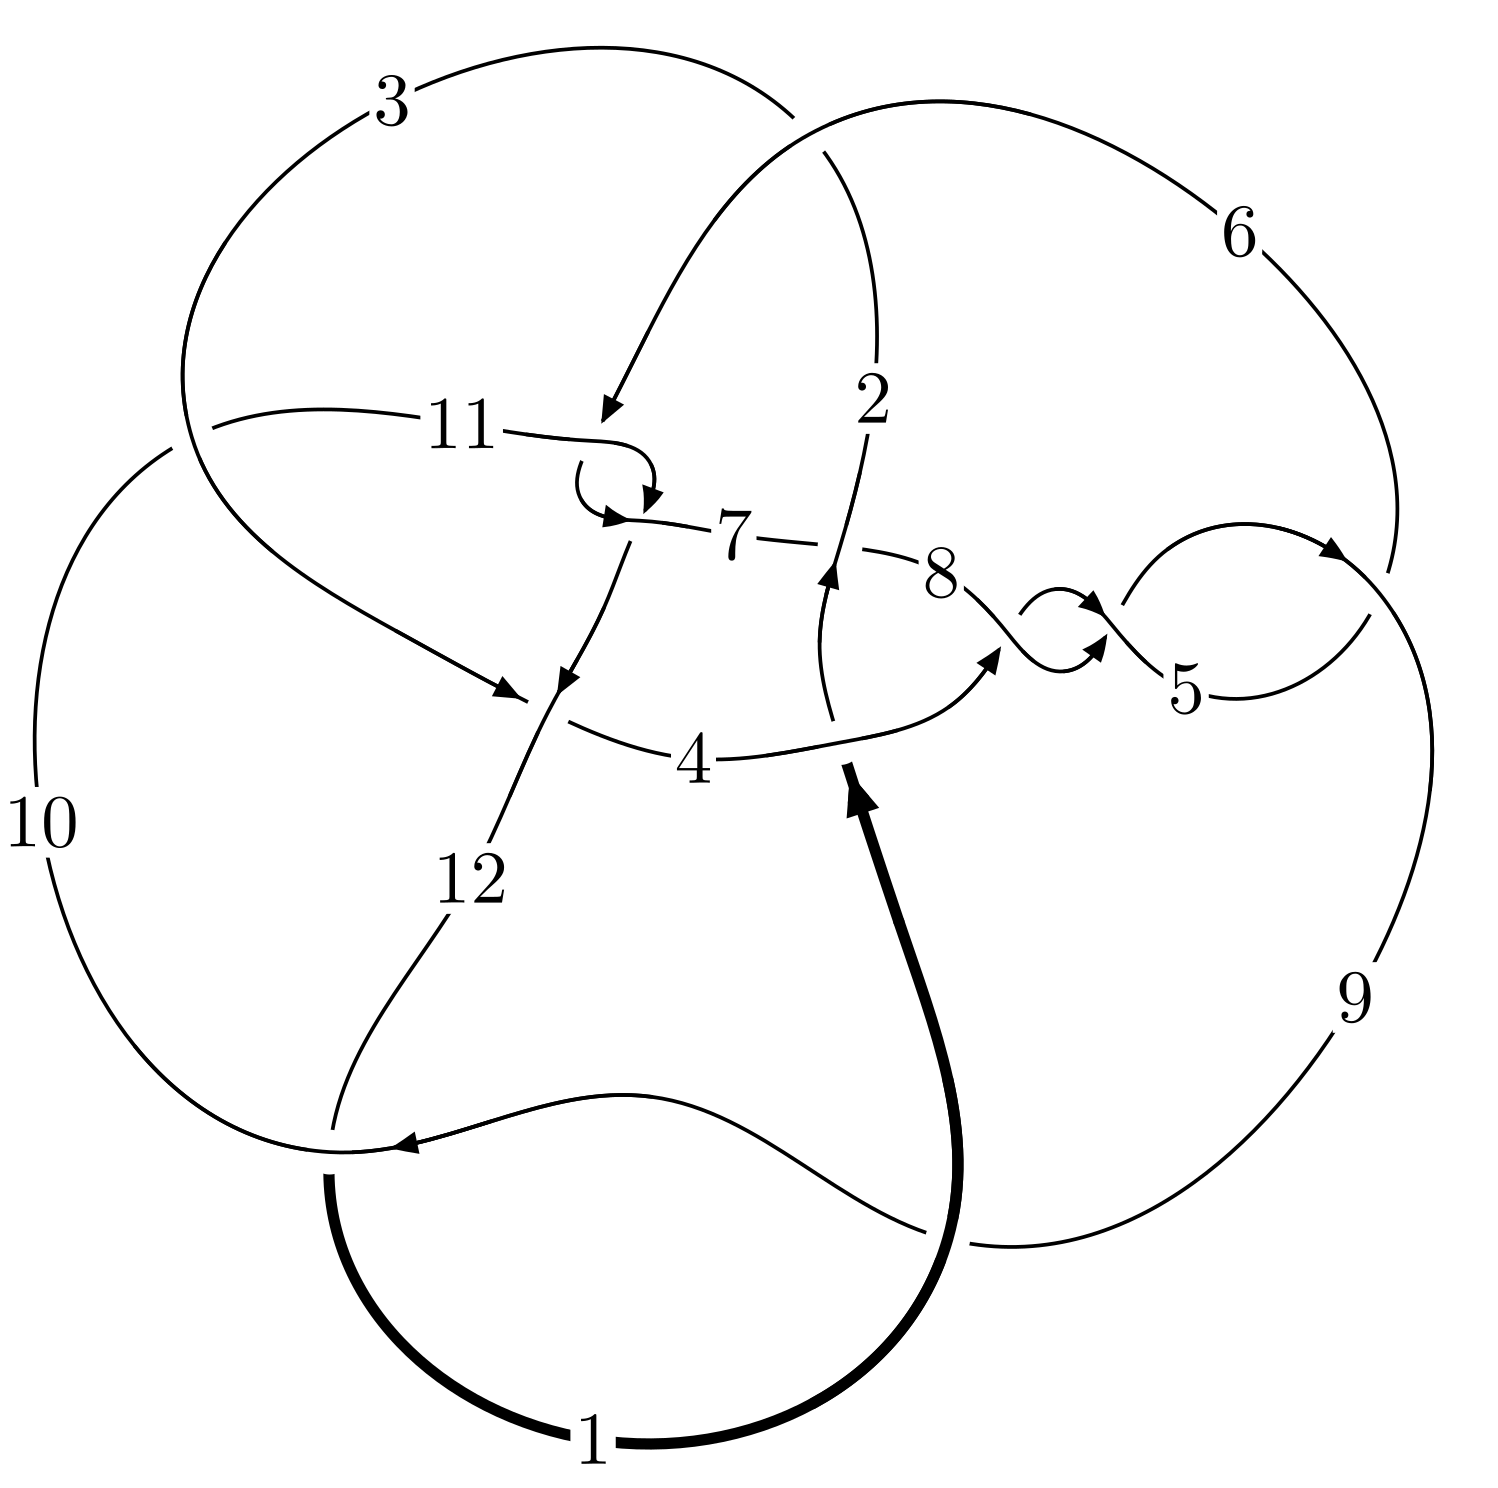
\includegraphics[width=112pt]{../../../GIT/diagram.site/Diagrams/png/1798_12a_0997.png}\\
\ \ \ A knot diagram\footnotemark}&
\allowdisplaybreaks
\textbf{Linearized knot diagam} \\
\cline{2-2}
 &
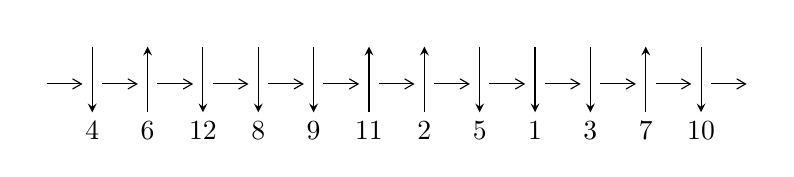
\begin{tikzpicture}[x=20pt, y=17pt]
	% nodes
	\node (C0) at (0, 0) {};
	\node (C1) at (1, 0) {};
	\node (C1U) at (1, +1) {};
	\node (C1D) at (1, -1) {4};

	\node (C2) at (2, 0) {};
	\node (C2U) at (2, +1) {};
	\node (C2D) at (2, -1) {6};

	\node (C3) at (3, 0) {};
	\node (C3U) at (3, +1) {};
	\node (C3D) at (3, -1) {12};

	\node (C4) at (4, 0) {};
	\node (C4U) at (4, +1) {};
	\node (C4D) at (4, -1) {8};

	\node (C5) at (5, 0) {};
	\node (C5U) at (5, +1) {};
	\node (C5D) at (5, -1) {9};

	\node (C6) at (6, 0) {};
	\node (C6U) at (6, +1) {};
	\node (C6D) at (6, -1) {11};

	\node (C7) at (7, 0) {};
	\node (C7U) at (7, +1) {};
	\node (C7D) at (7, -1) {2};

	\node (C8) at (8, 0) {};
	\node (C8U) at (8, +1) {};
	\node (C8D) at (8, -1) {5};

	\node (C9) at (9, 0) {};
	\node (C9U) at (9, +1) {};
	\node (C9D) at (9, -1) {1};

	\node (C10) at (10, 0) {};
	\node (C10U) at (10, +1) {};
	\node (C10D) at (10, -1) {3};

	\node (C11) at (11, 0) {};
	\node (C11U) at (11, +1) {};
	\node (C11D) at (11, -1) {7};

	\node (C12) at (12, 0) {};
	\node (C12U) at (12, +1) {};
	\node (C12D) at (12, -1) {10};
	\node (C13) at (13, 0) {};

	% arrows
	\draw[->,>={angle 60}]
	(C0) edge (C1) (C1) edge (C2) (C2) edge (C3) (C3) edge (C4) (C4) edge (C5) (C5) edge (C6) (C6) edge (C7) (C7) edge (C8) (C8) edge (C9) (C9) edge (C10) (C10) edge (C11) (C11) edge (C12) (C12) edge (C13) ;	\draw[->,>=stealth]
	(C1U) edge (C1D) (C2D) edge (C2U) (C3U) edge (C3D) (C4U) edge (C4D) (C5U) edge (C5D) (C6D) edge (C6U) (C7D) edge (C7U) (C8U) edge (C8D) (C9U) edge (C9D) (C10U) edge (C10D) (C11D) edge (C11U) (C12U) edge (C12D) ;
	\end{tikzpicture} \\
\hhline{~~} \\& 
\textbf{Solving Sequence} \\ \cline{2-2} 
 &
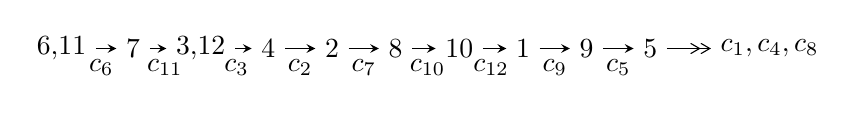
\begin{tikzpicture}[x=23pt, y=7pt]
	% node
	\node (A0) at (-1/8, 0) {6,11};
	\node (A1) at (1, 0) {7};
	\node (A2) at (33/16, 0) {3,12};
	\node (A3) at (25/8, 0) {4};
	\node (A4) at (33/8, 0) {2};
	\node (A5) at (41/8, 0) {8};
	\node (A6) at (49/8, 0) {10};
	\node (A7) at (57/8, 0) {1};
	\node (A8) at (65/8, 0) {9};
	\node (A9) at (73/8, 0) {5};
	\node (C1) at (1/2, -1) {$c_{6}$};
	\node (C2) at (3/2, -1) {$c_{11}$};
	\node (C3) at (21/8, -1) {$c_{3}$};
	\node (C4) at (29/8, -1) {$c_{2}$};
	\node (C5) at (37/8, -1) {$c_{7}$};
	\node (C6) at (45/8, -1) {$c_{10}$};
	\node (C7) at (53/8, -1) {$c_{12}$};
	\node (C8) at (61/8, -1) {$c_{9}$};
	\node (C9) at (69/8, -1) {$c_{5}$};
	\node (A10) at (11, 0) {$c_{1},c_{4},c_{8}$};

	% edge
	\draw[->,>=stealth]	
	(A0) edge (A1) (A1) edge (A2) (A2) edge (A3) (A3) edge (A4) (A4) edge (A5) (A5) edge (A6) (A6) edge (A7) (A7) edge (A8) (A8) edge (A9) ;
	\draw[->>,>={angle 60}]	
	(A9) edge (A10);
\end{tikzpicture} \\ 

\end{tabular} \\

\footnotetext{
The image of knot diagram is generated by the software ``\textbf{Draw programme}" developed by Andrew Bartholomew(\url{http://www.layer8.co.uk/maths/draw/index.htm\#Running-draw}), where we modified some parts for our purpose(\url{https://github.com/CATsTAILs/LinksPainter}).
}\phantom \\ \newline 
\centering \textbf{Ideals for irreducible components\footnotemark of $X_{\text{par}}$} 
 
\begin{align*}
I^u_{1}&=\langle 
-1.75024\times10^{474} u^{141}-1.96473\times10^{474} u^{140}+\cdots+4.83910\times10^{473} b-6.34671\times10^{476},\\
\phantom{I^u_{1}}&\phantom{= \langle  }-1.51920\times10^{476} u^{141}-1.86128\times10^{476} u^{140}+\cdots+2.95185\times10^{475} a-4.50856\times10^{478},\\
\phantom{I^u_{1}}&\phantom{= \langle  }u^{142}+2 u^{141}+\cdots+190 u+244\rangle \\
I^u_{2}&=\langle 
-113629468333922 u^{34}+73137569141391 u^{33}+\cdots+2341694541470 b-106088871052014,\\
\phantom{I^u_{2}}&\phantom{= \langle  }49505308067552 u^{34}-15174583421106 u^{33}+\cdots+2341694541470 a+131002690330904,\\
\phantom{I^u_{2}}&\phantom{= \langle  }u^{35}- u^{34}+\cdots+11 u^2-1\rangle \\
\\
\end{align*}
\raggedright * 2 irreducible components of $\dim_{\mathbb{C}}=0$, with total 177 representations.\\
\footnotetext{All coefficients of polynomials are rational numbers. But the coefficients are sometimes approximated in decimal forms when there is not enough margin.}
\newpage
\renewcommand{\arraystretch}{1}
\centering \section*{I. $I^u_{1}= \langle -1.75\times10^{474} u^{141}-1.96\times10^{474} u^{140}+\cdots+4.84\times10^{473} b-6.35\times10^{476},\;-1.52\times10^{476} u^{141}-1.86\times10^{476} u^{140}+\cdots+2.95\times10^{475} a-4.51\times10^{478},\;u^{142}+2 u^{141}+\cdots+190 u+244 \rangle$}
\flushleft \textbf{(i) Arc colorings}\\
\begin{tabular}{m{7pt} m{180pt} m{7pt} m{180pt} }
\flushright $a_{6}=$&$\begin{pmatrix}1\\0\end{pmatrix}$ \\
\flushright $a_{11}=$&$\begin{pmatrix}0\\u\end{pmatrix}$ \\
\flushright $a_{7}=$&$\begin{pmatrix}1\\- u^2\end{pmatrix}$ \\
\flushright $a_{3}=$&$\begin{pmatrix}5.14659 u^{141}+6.30546 u^{140}+\cdots-696.725 u+1527.37\\3.61686 u^{141}+4.06012 u^{140}+\cdots-365.894 u+1311.55\end{pmatrix}$ \\
\flushright $a_{12}=$&$\begin{pmatrix}u\\- u^3+u\end{pmatrix}$ \\
\flushright $a_{4}=$&$\begin{pmatrix}4.46182 u^{141}+5.51814 u^{140}+\cdots-619.473 u+1177.84\\3.21273 u^{141}+3.71733 u^{140}+\cdots-345.106 u+1104.07\end{pmatrix}$ \\
\flushright $a_{2}=$&$\begin{pmatrix}1.52972 u^{141}+2.24534 u^{140}+\cdots-330.831 u+215.820\\3.61686 u^{141}+4.06012 u^{140}+\cdots-365.894 u+1311.55\end{pmatrix}$ \\
\flushright $a_{8}=$&$\begin{pmatrix}-4.11774 u^{141}-6.11606 u^{140}+\cdots+1329.29 u-1495.35\\0.246365 u^{141}+0.0837458 u^{140}+\cdots+332.526 u-91.8020\end{pmatrix}$ \\
\flushright $a_{10}=$&$\begin{pmatrix}-3.83345 u^{141}-5.21359 u^{140}+\cdots+1191.52 u-1902.87\\-0.981164 u^{141}-1.78349 u^{140}+\cdots+589.787 u-389.643\end{pmatrix}$ \\
\flushright $a_{1}=$&$\begin{pmatrix}-9.93857 u^{141}-12.6394 u^{140}+\cdots+2116.16 u-3531.76\\-2.69583 u^{141}-3.60343 u^{140}+\cdots+725.805 u-921.068\end{pmatrix}$ \\
\flushright $a_{9}=$&$\begin{pmatrix}-11.1461 u^{141}-15.0882 u^{140}+\cdots+2795.38 u-3894.61\\-3.09865 u^{141}-4.28797 u^{140}+\cdots+956.752 u-1211.52\end{pmatrix}$ \\
\flushright $a_{5}=$&$\begin{pmatrix}10.6780 u^{141}+14.6267 u^{140}+\cdots-2679.81 u+3654.33\\-1.37124 u^{141}-1.90190 u^{140}+\cdots+326.354 u-382.690\end{pmatrix}$\\&\end{tabular}
\flushleft \textbf{(ii) Obstruction class $= -1$}\\~\\
\flushleft \textbf{(iii) Cusp Shapes $= 3.69920 u^{141}+6.20634 u^{140}+\cdots-2253.29 u+1903.17$}\\~\\
\newpage\renewcommand{\arraystretch}{1}
\flushleft \textbf{(iv) u-Polynomials at the component}\newline \\
\begin{tabular}{m{50pt}|m{274pt}}
Crossings & \hspace{64pt}u-Polynomials at each crossing \\
\hline $$\begin{aligned}c_{1}\end{aligned}$$&$\begin{aligned}
&u^{142}+3 u^{141}+\cdots-5484992 u-358484
\end{aligned}$\\
\hline $$\begin{aligned}c_{2}\end{aligned}$$&$\begin{aligned}
&u^{142}+4 u^{141}+\cdots+287961643 u+41067731
\end{aligned}$\\
\hline $$\begin{aligned}c_{3}\end{aligned}$$&$\begin{aligned}
&u^{142}-2 u^{141}+\cdots+113943 u-4559
\end{aligned}$\\
\hline $$\begin{aligned}c_{4},c_{5},c_{8}\end{aligned}$$&$\begin{aligned}
&u^{142}+4 u^{141}+\cdots+659 u-79
\end{aligned}$\\
\hline $$\begin{aligned}c_{6},c_{11}\end{aligned}$$&$\begin{aligned}
&u^{142}+2 u^{141}+\cdots+190 u+244
\end{aligned}$\\
\hline $$\begin{aligned}c_{7}\end{aligned}$$&$\begin{aligned}
&u^{142}+u^{141}+\cdots-118669 u-6359
\end{aligned}$\\
\hline $$\begin{aligned}c_{9},c_{12}\end{aligned}$$&$\begin{aligned}
&u^{142}-9 u^{141}+\cdots+352548 u-24091
\end{aligned}$\\
\hline $$\begin{aligned}c_{10}\end{aligned}$$&$\begin{aligned}
&u^{142}-2 u^{141}+\cdots+64376759 u-5349403
\end{aligned}$\\
\hline
\end{tabular}\\~\\
\newpage\renewcommand{\arraystretch}{1}
\flushleft \textbf{(v) Riley Polynomials at the component}\newline \\
\begin{tabular}{m{50pt}|m{274pt}}
Crossings & \hspace{64pt}Riley Polynomials at each crossing \\
\hline $$\begin{aligned}c_{1}\end{aligned}$$&$\begin{aligned}
&y^{142}-19 y^{141}+\cdots-3842346849688 y+128510778256
\end{aligned}$\\
\hline $$\begin{aligned}c_{2}\end{aligned}$$&$\begin{aligned}
&y^{142}-20 y^{141}+\cdots-70044640456027673 y+1686558529488361
\end{aligned}$\\
\hline $$\begin{aligned}c_{3}\end{aligned}$$&$\begin{aligned}
&y^{142}+46 y^{141}+\cdots-4311752777 y+20784481
\end{aligned}$\\
\hline $$\begin{aligned}c_{4},c_{5},c_{8}\end{aligned}$$&$\begin{aligned}
&y^{142}-136 y^{141}+\cdots+195349 y+6241
\end{aligned}$\\
\hline $$\begin{aligned}c_{6},c_{11}\end{aligned}$$&$\begin{aligned}
&y^{142}-86 y^{141}+\cdots-1799244 y+59536
\end{aligned}$\\
\hline $$\begin{aligned}c_{7}\end{aligned}$$&$\begin{aligned}
&y^{142}+43 y^{141}+\cdots+7868694797 y+40436881
\end{aligned}$\\
\hline $$\begin{aligned}c_{9},c_{12}\end{aligned}$$&$\begin{aligned}
&y^{142}+103 y^{141}+\cdots+15947376892 y+580376281
\end{aligned}$\\
\hline $$\begin{aligned}c_{10}\end{aligned}$$&$\begin{aligned}
&y^{142}+48 y^{141}+\cdots+1001793325679001 y+28616112456409
\end{aligned}$\\
\hline
\end{tabular}\\~\\
\newpage\flushleft \textbf{(vi) Complex Volumes and Cusp Shapes}
$$\begin{array}{c|c|c}  
\text{Solutions to }I^u_{1}& \I (\text{vol} + \sqrt{-1}CS) & \text{Cusp shape}\\
 \hline 
\begin{aligned}
u &= -0.295441 + 0.961168 I \\
a &= \phantom{-}0.669363 - 0.698149 I \\
b &= \phantom{-}1.305230 - 0.036216 I\end{aligned}
 & -1.64573 - 4.86259 I & \phantom{-0.000000 } 0 \\ \hline\begin{aligned}
u &= -0.295441 - 0.961168 I \\
a &= \phantom{-}0.669363 + 0.698149 I \\
b &= \phantom{-}1.305230 + 0.036216 I\end{aligned}
 & -1.64573 + 4.86259 I & \phantom{-0.000000 } 0 \\ \hline\begin{aligned}
u &= \phantom{-}0.995761 + 0.156820 I \\
a &= -0.222456 + 0.767537 I \\
b &= -0.83941 + 2.00273 I\end{aligned}
 & \phantom{-}3.44526 + 4.94912 I & \phantom{-0.000000 } 0 \\ \hline\begin{aligned}
u &= \phantom{-}0.995761 - 0.156820 I \\
a &= -0.222456 - 0.767537 I \\
b &= -0.83941 - 2.00273 I\end{aligned}
 & \phantom{-}3.44526 - 4.94912 I & \phantom{-0.000000 } 0 \\ \hline\begin{aligned}
u &= -1.012530 + 0.042524 I \\
a &= -0.316472 + 0.782864 I \\
b &= \phantom{-}1.82554 + 0.66888 I\end{aligned}
 & \phantom{-}5.66183 - 0.09728 I & \phantom{-0.000000 } 0 \\ \hline\begin{aligned}
u &= -1.012530 - 0.042524 I \\
a &= -0.316472 - 0.782864 I \\
b &= \phantom{-}1.82554 - 0.66888 I\end{aligned}
 & \phantom{-}5.66183 + 0.09728 I & \phantom{-0.000000 } 0 \\ \hline\begin{aligned}
u &= -0.960789 + 0.327128 I \\
a &= -1.67573 - 0.53788 I \\
b &= \phantom{-}0.573811 - 0.699430 I\end{aligned}
 & \phantom{-}2.24599 - 6.21367 I & \phantom{-0.000000 } 0 \\ \hline\begin{aligned}
u &= -0.960789 - 0.327128 I \\
a &= -1.67573 + 0.53788 I \\
b &= \phantom{-}0.573811 + 0.699430 I\end{aligned}
 & \phantom{-}2.24599 + 6.21367 I & \phantom{-0.000000 } 0 \\ \hline\begin{aligned}
u &= \phantom{-}0.905560 + 0.387213 I \\
a &= \phantom{-}1.117890 - 0.286171 I \\
b &= -0.333646 - 0.244719 I\end{aligned}
 & \phantom{-}1.65458 + 2.59253 I & \phantom{-0.000000 } 0 \\ \hline\begin{aligned}
u &= \phantom{-}0.905560 - 0.387213 I \\
a &= \phantom{-}1.117890 + 0.286171 I \\
b &= -0.333646 + 0.244719 I\end{aligned}
 & \phantom{-}1.65458 - 2.59253 I & \phantom{-0.000000 } 0\\
 \hline 
 \end{array}$$\newpage$$\begin{array}{c|c|c}  
\text{Solutions to }I^u_{1}& \I (\text{vol} + \sqrt{-1}CS) & \text{Cusp shape}\\
 \hline 
\begin{aligned}
u &= -0.665433 + 0.773073 I \\
a &= \phantom{-}0.227227 - 0.578619 I \\
b &= \phantom{-}0.927867 + 0.531487 I\end{aligned}
 & -0.77924 - 1.97467 I & \phantom{-0.000000 } 0 \\ \hline\begin{aligned}
u &= -0.665433 - 0.773073 I \\
a &= \phantom{-}0.227227 + 0.578619 I \\
b &= \phantom{-}0.927867 - 0.531487 I\end{aligned}
 & -0.77924 + 1.97467 I & \phantom{-0.000000 } 0 \\ \hline\begin{aligned}
u &= \phantom{-}0.947015 + 0.184346 I \\
a &= -1.53370 - 0.54169 I \\
b &= \phantom{-}0.689578 + 0.125937 I\end{aligned}
 & \phantom{-}0.06734 + 2.02026 I & \phantom{-0.000000 } 0 \\ \hline\begin{aligned}
u &= \phantom{-}0.947015 - 0.184346 I \\
a &= -1.53370 + 0.54169 I \\
b &= \phantom{-}0.689578 - 0.125937 I\end{aligned}
 & \phantom{-}0.06734 - 2.02026 I & \phantom{-0.000000 } 0 \\ \hline\begin{aligned}
u &= \phantom{-}0.991552 + 0.329410 I \\
a &= \phantom{-}2.02454 - 0.43908 I \\
b &= -0.511332 - 0.970263 I\end{aligned}
 & -3.51611 + 9.45267 I & \phantom{-0.000000 } 0 \\ \hline\begin{aligned}
u &= \phantom{-}0.991552 - 0.329410 I \\
a &= \phantom{-}2.02454 + 0.43908 I \\
b &= -0.511332 + 0.970263 I\end{aligned}
 & -3.51611 - 9.45267 I & \phantom{-0.000000 } 0 \\ \hline\begin{aligned}
u &= -1.022900 + 0.233568 I \\
a &= \phantom{-}1.59300 - 0.86822 I \\
b &= -0.534375 + 0.348376 I\end{aligned}
 & -4.94516 - 4.59022 I & \phantom{-0.000000 } 0 \\ \hline\begin{aligned}
u &= -1.022900 - 0.233568 I \\
a &= \phantom{-}1.59300 + 0.86822 I \\
b &= -0.534375 - 0.348376 I\end{aligned}
 & -4.94516 + 4.59022 I & \phantom{-0.000000 } 0 \\ \hline\begin{aligned}
u &= -0.949398\phantom{ +0.000000I} \\
a &= \phantom{-}1.81107\phantom{ +0.000000I} \\
b &= -0.915073\phantom{ +0.000000I}\end{aligned}
 & -2.43501\phantom{ +0.000000I} & \phantom{-0.000000 } 0 \\ \hline\begin{aligned}
u &= \phantom{-}0.940257 + 0.110353 I \\
a &= \phantom{-}0.877495 - 1.020720 I \\
b &= -1.365760 - 0.120797 I\end{aligned}
 & \phantom{-}1.99013 + 3.91057 I & \phantom{-0.000000 } 0\\
 \hline 
 \end{array}$$\newpage$$\begin{array}{c|c|c}  
\text{Solutions to }I^u_{1}& \I (\text{vol} + \sqrt{-1}CS) & \text{Cusp shape}\\
 \hline 
\begin{aligned}
u &= \phantom{-}0.940257 - 0.110353 I \\
a &= \phantom{-}0.877495 + 1.020720 I \\
b &= -1.365760 + 0.120797 I\end{aligned}
 & \phantom{-}1.99013 - 3.91057 I & \phantom{-0.000000 } 0 \\ \hline\begin{aligned}
u &= -0.977297 + 0.445677 I \\
a &= -1.242200 + 0.390383 I \\
b &= -0.255815 - 0.424907 I\end{aligned}
 & -4.14393 - 0.12942 I & \phantom{-0.000000 } 0 \\ \hline\begin{aligned}
u &= -0.977297 - 0.445677 I \\
a &= -1.242200 - 0.390383 I \\
b &= -0.255815 + 0.424907 I\end{aligned}
 & -4.14393 + 0.12942 I & \phantom{-0.000000 } 0 \\ \hline\begin{aligned}
u &= \phantom{-}0.939586 + 0.533139 I \\
a &= -1.026660 - 0.963608 I \\
b &= -0.289039 - 0.097357 I\end{aligned}
 & -3.18828 - 1.94077 I & \phantom{-0.000000 } 0 \\ \hline\begin{aligned}
u &= \phantom{-}0.939586 - 0.533139 I \\
a &= -1.026660 + 0.963608 I \\
b &= -0.289039 + 0.097357 I\end{aligned}
 & -3.18828 + 1.94077 I & \phantom{-0.000000 } 0 \\ \hline\begin{aligned}
u &= \phantom{-}0.952349 + 0.526982 I \\
a &= -0.889049 - 0.707415 I \\
b &= -1.382320 + 0.276137 I\end{aligned}
 & \phantom{-}2.18933 - 1.03709 I & \phantom{-0.000000 } 0 \\ \hline\begin{aligned}
u &= \phantom{-}0.952349 - 0.526982 I \\
a &= -0.889049 + 0.707415 I \\
b &= -1.382320 - 0.276137 I\end{aligned}
 & \phantom{-}2.18933 + 1.03709 I & \phantom{-0.000000 } 0 \\ \hline\begin{aligned}
u &= \phantom{-}0.180527 + 0.888125 I \\
a &= -0.901850 + 0.760556 I \\
b &= -0.249599 + 1.045440 I\end{aligned}
 & -7.35446 - 1.74290 I & \phantom{-0.000000 } 0 \\ \hline\begin{aligned}
u &= \phantom{-}0.180527 - 0.888125 I \\
a &= -0.901850 - 0.760556 I \\
b &= -0.249599 - 1.045440 I\end{aligned}
 & -7.35446 + 1.74290 I & \phantom{-0.000000 } 0 \\ \hline\begin{aligned}
u &= -0.863621 + 0.269420 I \\
a &= \phantom{-}0.038865 - 0.642852 I \\
b &= -0.412835 - 1.143140 I\end{aligned}
 & -0.89229 - 2.62212 I & \phantom{-0.000000 } 0\\
 \hline 
 \end{array}$$\newpage$$\begin{array}{c|c|c}  
\text{Solutions to }I^u_{1}& \I (\text{vol} + \sqrt{-1}CS) & \text{Cusp shape}\\
 \hline 
\begin{aligned}
u &= -0.863621 - 0.269420 I \\
a &= \phantom{-}0.038865 + 0.642852 I \\
b &= -0.412835 + 1.143140 I\end{aligned}
 & -0.89229 + 2.62212 I & \phantom{-0.000000 } 0 \\ \hline\begin{aligned}
u &= -0.096232 + 1.094430 I \\
a &= \phantom{-}0.887299 + 0.457796 I \\
b &= \phantom{-}0.676233 + 0.624368 I\end{aligned}
 & \phantom{-}1.03726 + 3.47735 I & \phantom{-0.000000 } 0 \\ \hline\begin{aligned}
u &= -0.096232 - 1.094430 I \\
a &= \phantom{-}0.887299 - 0.457796 I \\
b &= \phantom{-}0.676233 - 0.624368 I\end{aligned}
 & \phantom{-}1.03726 - 3.47735 I & \phantom{-0.000000 } 0 \\ \hline\begin{aligned}
u &= -0.867137 + 0.227443 I \\
a &= \phantom{-}0.664833 + 0.617823 I \\
b &= -0.01210 + 2.70109 I\end{aligned}
 & -4.02573 - 8.08694 I & \phantom{-0.000000 } 0 \\ \hline\begin{aligned}
u &= -0.867137 - 0.227443 I \\
a &= \phantom{-}0.664833 - 0.617823 I \\
b &= -0.01210 - 2.70109 I\end{aligned}
 & -4.02573 + 8.08694 I & \phantom{-0.000000 } 0 \\ \hline\begin{aligned}
u &= \phantom{-}0.156814 + 1.098300 I \\
a &= -1.030160 + 0.457830 I \\
b &= -0.943074 + 0.722792 I\end{aligned}
 & \phantom{-}2.45324 - 8.83016 I & \phantom{-0.000000 } 0 \\ \hline\begin{aligned}
u &= \phantom{-}0.156814 - 1.098300 I \\
a &= -1.030160 - 0.457830 I \\
b &= -0.943074 - 0.722792 I\end{aligned}
 & \phantom{-}2.45324 + 8.83016 I & \phantom{-0.000000 } 0 \\ \hline\begin{aligned}
u &= -0.177578 + 1.097880 I \\
a &= \phantom{-}1.098380 + 0.499845 I \\
b &= \phantom{-}1.080490 + 0.868581 I\end{aligned}
 & -3.56242 + 13.15990 I & \phantom{-0.000000 } 0 \\ \hline\begin{aligned}
u &= -0.177578 - 1.097880 I \\
a &= \phantom{-}1.098380 - 0.499845 I \\
b &= \phantom{-}1.080490 - 0.868581 I\end{aligned}
 & -3.56242 - 13.15990 I & \phantom{-0.000000 } 0 \\ \hline\begin{aligned}
u &= \phantom{-}0.801356 + 0.357639 I \\
a &= \phantom{-}0.211805 - 0.263722 I \\
b &= \phantom{-}0.55333 - 1.69086 I\end{aligned}
 & -7.22523 + 4.37051 I & \phantom{-0.000000 } 0\\
 \hline 
 \end{array}$$\newpage$$\begin{array}{c|c|c}  
\text{Solutions to }I^u_{1}& \I (\text{vol} + \sqrt{-1}CS) & \text{Cusp shape}\\
 \hline 
\begin{aligned}
u &= \phantom{-}0.801356 - 0.357639 I \\
a &= \phantom{-}0.211805 + 0.263722 I \\
b &= \phantom{-}0.55333 + 1.69086 I\end{aligned}
 & -7.22523 - 4.37051 I & \phantom{-0.000000 } 0 \\ \hline\begin{aligned}
u &= -0.677192 + 0.532116 I \\
a &= \phantom{-}1.22550 - 0.89397 I \\
b &= \phantom{-}0.325908 - 0.517957 I\end{aligned}
 & \phantom{-}0.49068 - 2.16297 I & \phantom{-0.000000 } 0 \\ \hline\begin{aligned}
u &= -0.677192 - 0.532116 I \\
a &= \phantom{-}1.22550 + 0.89397 I \\
b &= \phantom{-}0.325908 + 0.517957 I\end{aligned}
 & \phantom{-}0.49068 + 2.16297 I & \phantom{-0.000000 } 0 \\ \hline\begin{aligned}
u &= -0.253184 + 1.118540 I \\
a &= -0.645230 - 0.209736 I \\
b &= -0.742559 - 0.446593 I\end{aligned}
 & -1.78631 + 3.15535 I & \phantom{-0.000000 } 0 \\ \hline\begin{aligned}
u &= -0.253184 - 1.118540 I \\
a &= -0.645230 + 0.209736 I \\
b &= -0.742559 + 0.446593 I\end{aligned}
 & -1.78631 - 3.15535 I & \phantom{-0.000000 } 0 \\ \hline\begin{aligned}
u &= -0.775010 + 0.335653 I \\
a &= -1.49027 - 0.18784 I \\
b &= \phantom{-}1.03264 - 1.59318 I\end{aligned}
 & -4.12735 + 5.42432 I & \phantom{-0.000000 } 0 \\ \hline\begin{aligned}
u &= -0.775010 - 0.335653 I \\
a &= -1.49027 + 0.18784 I \\
b &= \phantom{-}1.03264 + 1.59318 I\end{aligned}
 & -4.12735 - 5.42432 I & \phantom{-0.000000 } 0 \\ \hline\begin{aligned}
u &= \phantom{-}0.381711 + 0.747319 I \\
a &= -0.508385 - 0.935626 I \\
b &= -1.030840 + 0.114718 I\end{aligned}
 & \phantom{-}3.08868 + 3.12603 I & \phantom{-0.000000 } 0 \\ \hline\begin{aligned}
u &= \phantom{-}0.381711 - 0.747319 I \\
a &= -0.508385 + 0.935626 I \\
b &= -1.030840 - 0.114718 I\end{aligned}
 & \phantom{-}3.08868 - 3.12603 I & \phantom{-0.000000 } 0 \\ \hline\begin{aligned}
u &= \phantom{-}0.677307 + 0.479418 I \\
a &= -0.959029 + 0.608697 I \\
b &= \phantom{-}1.147290 + 0.688353 I\end{aligned}
 & -7.48981 - 0.76566 I & \phantom{-0.000000 } 0\\
 \hline 
 \end{array}$$\newpage$$\begin{array}{c|c|c}  
\text{Solutions to }I^u_{1}& \I (\text{vol} + \sqrt{-1}CS) & \text{Cusp shape}\\
 \hline 
\begin{aligned}
u &= \phantom{-}0.677307 - 0.479418 I \\
a &= -0.959029 - 0.608697 I \\
b &= \phantom{-}1.147290 - 0.688353 I\end{aligned}
 & -7.48981 + 0.76566 I & \phantom{-0.000000 } 0 \\ \hline\begin{aligned}
u &= \phantom{-}0.439527 + 1.097660 I \\
a &= \phantom{-}0.531971 - 0.006531 I \\
b &= \phantom{-}0.431681 - 0.279722 I\end{aligned}
 & -1.32780 + 1.36080 I & \phantom{-0.000000 } 0 \\ \hline\begin{aligned}
u &= \phantom{-}0.439527 - 1.097660 I \\
a &= \phantom{-}0.531971 + 0.006531 I \\
b &= \phantom{-}0.431681 + 0.279722 I\end{aligned}
 & -1.32780 - 1.36080 I & \phantom{-0.000000 } 0 \\ \hline\begin{aligned}
u &= -1.073910 + 0.509333 I \\
a &= \phantom{-}0.435785 - 0.982606 I \\
b &= \phantom{-}1.47076 - 0.00231 I\end{aligned}
 & \phantom{-}6.39536 - 1.71581 I & \phantom{-0.000000 } 0 \\ \hline\begin{aligned}
u &= -1.073910 - 0.509333 I \\
a &= \phantom{-}0.435785 + 0.982606 I \\
b &= \phantom{-}1.47076 + 0.00231 I\end{aligned}
 & \phantom{-}6.39536 + 1.71581 I & \phantom{-0.000000 } 0 \\ \hline\begin{aligned}
u &= -1.102960 + 0.455345 I \\
a &= \phantom{-}0.53637 + 1.53987 I \\
b &= -1.44783 + 1.60931 I\end{aligned}
 & \phantom{-}2.40570 - 7.60763 I & \phantom{-0.000000 } 0 \\ \hline\begin{aligned}
u &= -1.102960 - 0.455345 I \\
a &= \phantom{-}0.53637 - 1.53987 I \\
b &= -1.44783 - 1.60931 I\end{aligned}
 & \phantom{-}2.40570 + 7.60763 I & \phantom{-0.000000 } 0 \\ \hline\begin{aligned}
u &= \phantom{-}0.788812 + 0.129788 I \\
a &= -0.03648 - 1.50672 I \\
b &= \phantom{-}0.329050 - 0.928368 I\end{aligned}
 & -0.490370 - 0.236987 I & \phantom{-0.000000 } 0 \\ \hline\begin{aligned}
u &= \phantom{-}0.788812 - 0.129788 I \\
a &= -0.03648 + 1.50672 I \\
b &= \phantom{-}0.329050 + 0.928368 I\end{aligned}
 & -0.490370 + 0.236987 I & \phantom{-0.000000 } 0 \\ \hline\begin{aligned}
u &= \phantom{-}1.143600 + 0.423408 I \\
a &= -0.055369 - 1.256870 I \\
b &= -1.62856 - 0.22646 I\end{aligned}
 & \phantom{-}2.78962 + 4.09503 I & \phantom{-0.000000 } 0\\
 \hline 
 \end{array}$$\newpage$$\begin{array}{c|c|c}  
\text{Solutions to }I^u_{1}& \I (\text{vol} + \sqrt{-1}CS) & \text{Cusp shape}\\
 \hline 
\begin{aligned}
u &= \phantom{-}1.143600 - 0.423408 I \\
a &= -0.055369 + 1.256870 I \\
b &= -1.62856 + 0.22646 I\end{aligned}
 & \phantom{-}2.78962 - 4.09503 I & \phantom{-0.000000 } 0 \\ \hline\begin{aligned}
u &= \phantom{-}1.161030 + 0.373280 I \\
a &= \phantom{-}0.547399 - 0.852433 I \\
b &= -1.40420 - 1.35000 I\end{aligned}
 & -2.98025 + 6.85607 I & \phantom{-0.000000 } 0 \\ \hline\begin{aligned}
u &= \phantom{-}1.161030 - 0.373280 I \\
a &= \phantom{-}0.547399 + 0.852433 I \\
b &= -1.40420 + 1.35000 I\end{aligned}
 & -2.98025 - 6.85607 I & \phantom{-0.000000 } 0 \\ \hline\begin{aligned}
u &= -1.192180 + 0.266198 I \\
a &= \phantom{-}0.119991 + 0.494450 I \\
b &= -2.15150 + 1.08202 I\end{aligned}
 & -0.46667 - 8.68353 I & \phantom{-0.000000 } 0 \\ \hline\begin{aligned}
u &= -1.192180 - 0.266198 I \\
a &= \phantom{-}0.119991 - 0.494450 I \\
b &= -2.15150 - 1.08202 I\end{aligned}
 & -0.46667 + 8.68353 I & \phantom{-0.000000 } 0 \\ \hline\begin{aligned}
u &= \phantom{-}1.204900 + 0.248316 I \\
a &= -0.216469 + 1.272930 I \\
b &= \phantom{-}0.247465 + 0.663571 I\end{aligned}
 & \phantom{-}4.55521 + 4.15623 I & \phantom{-0.000000 } 0 \\ \hline\begin{aligned}
u &= \phantom{-}1.204900 - 0.248316 I \\
a &= -0.216469 - 1.272930 I \\
b &= \phantom{-}0.247465 - 0.663571 I\end{aligned}
 & \phantom{-}4.55521 - 4.15623 I & \phantom{-0.000000 } 0 \\ \hline\begin{aligned}
u &= \phantom{-}1.157320 + 0.444718 I \\
a &= -0.33903 + 1.52701 I \\
b &= \phantom{-}1.41902 + 1.12486 I\end{aligned}
 & \phantom{-}6.68328 + 6.03023 I & \phantom{-0.000000 } 0 \\ \hline\begin{aligned}
u &= \phantom{-}1.157320 - 0.444718 I \\
a &= -0.33903 - 1.52701 I \\
b &= \phantom{-}1.41902 - 1.12486 I\end{aligned}
 & \phantom{-}6.68328 - 6.03023 I & \phantom{-0.000000 } 0 \\ \hline\begin{aligned}
u &= -0.104805 + 0.742473 I \\
a &= -1.63727 - 0.49313 I \\
b &= -1.315660 - 0.362701 I\end{aligned}
 & -0.759364 - 0.251461 I & \phantom{-0.000000 } 0\\
 \hline 
 \end{array}$$\newpage$$\begin{array}{c|c|c}  
\text{Solutions to }I^u_{1}& \I (\text{vol} + \sqrt{-1}CS) & \text{Cusp shape}\\
 \hline 
\begin{aligned}
u &= -0.104805 - 0.742473 I \\
a &= -1.63727 + 0.49313 I \\
b &= -1.315660 + 0.362701 I\end{aligned}
 & -0.759364 + 0.251461 I & \phantom{-0.000000 } 0 \\ \hline\begin{aligned}
u &= \phantom{-}0.203821 + 1.238700 I \\
a &= \phantom{-}0.563722 - 0.312244 I \\
b &= \phantom{-}0.797764 - 0.681525 I\end{aligned}
 & -8.34882 - 6.21982 I & \phantom{-0.000000 } 0 \\ \hline\begin{aligned}
u &= \phantom{-}0.203821 - 1.238700 I \\
a &= \phantom{-}0.563722 + 0.312244 I \\
b &= \phantom{-}0.797764 + 0.681525 I\end{aligned}
 & -8.34882 + 6.21982 I & \phantom{-0.000000 } 0 \\ \hline\begin{aligned}
u &= -1.203770 + 0.363815 I \\
a &= -0.352127 - 0.887998 I \\
b &= \phantom{-}1.13437 - 0.84632 I\end{aligned}
 & \phantom{-}3.52882 - 4.29863 I & \phantom{-0.000000 } 0 \\ \hline\begin{aligned}
u &= -1.203770 - 0.363815 I \\
a &= -0.352127 + 0.887998 I \\
b &= \phantom{-}1.13437 + 0.84632 I\end{aligned}
 & \phantom{-}3.52882 + 4.29863 I & \phantom{-0.000000 } 0 \\ \hline\begin{aligned}
u &= -0.726023 + 0.057363 I \\
a &= -0.02709 - 2.28085 I \\
b &= -0.408026 - 1.136080 I\end{aligned}
 & -6.24327 + 2.81788 I & \phantom{-0.000000 } 0 \\ \hline\begin{aligned}
u &= -0.726023 - 0.057363 I \\
a &= -0.02709 + 2.28085 I \\
b &= -0.408026 + 1.136080 I\end{aligned}
 & -6.24327 - 2.81788 I & \phantom{-0.000000 } 0 \\ \hline\begin{aligned}
u &= -1.182400 + 0.477988 I \\
a &= \phantom{-}0.15640 + 1.62156 I \\
b &= -1.67251 + 0.78530 I\end{aligned}
 & \phantom{-}2.38272 - 4.27099 I & \phantom{-0.000000 } 0 \\ \hline\begin{aligned}
u &= -1.182400 - 0.477988 I \\
a &= \phantom{-}0.15640 - 1.62156 I \\
b &= -1.67251 - 0.78530 I\end{aligned}
 & \phantom{-}2.38272 + 4.27099 I & \phantom{-0.000000 } 0 \\ \hline\begin{aligned}
u &= -1.257260 + 0.347278 I \\
a &= \phantom{-}0.257115 + 1.341720 I \\
b &= -0.849485 + 0.541354 I\end{aligned}
 & \phantom{-}7.71716 - 6.70943 I & \phantom{-0.000000 } 0\\
 \hline 
 \end{array}$$\newpage$$\begin{array}{c|c|c}  
\text{Solutions to }I^u_{1}& \I (\text{vol} + \sqrt{-1}CS) & \text{Cusp shape}\\
 \hline 
\begin{aligned}
u &= -1.257260 - 0.347278 I \\
a &= \phantom{-}0.257115 - 1.341720 I \\
b &= -0.849485 - 0.541354 I\end{aligned}
 & \phantom{-}7.71716 + 6.70943 I & \phantom{-0.000000 } 0 \\ \hline\begin{aligned}
u &= \phantom{-}1.298120 + 0.128170 I \\
a &= \phantom{-}0.041391 + 0.468615 I \\
b &= \phantom{-}1.30327 + 1.66542 I\end{aligned}
 & \phantom{-}6.24725 + 3.31596 I & \phantom{-0.000000 } 0 \\ \hline\begin{aligned}
u &= \phantom{-}1.298120 - 0.128170 I \\
a &= \phantom{-}0.041391 - 0.468615 I \\
b &= \phantom{-}1.30327 - 1.66542 I\end{aligned}
 & \phantom{-}6.24725 - 3.31596 I & \phantom{-0.000000 } 0 \\ \hline\begin{aligned}
u &= -0.519635 + 1.211370 I \\
a &= -0.345095 - 0.080928 I \\
b &= -0.137004 - 0.488716 I\end{aligned}
 & -7.75612 - 5.05750 I & \phantom{-0.000000 } 0 \\ \hline\begin{aligned}
u &= -0.519635 - 1.211370 I \\
a &= -0.345095 + 0.080928 I \\
b &= -0.137004 + 0.488716 I\end{aligned}
 & -7.75612 + 5.05750 I & \phantom{-0.000000 } 0 \\ \hline\begin{aligned}
u &= \phantom{-}0.296596 + 0.613764 I \\
a &= \phantom{-}0.216062 + 1.144900 I \\
b &= -0.097240 + 0.765571 I\end{aligned}
 & \phantom{-}0.050700 + 1.129900 I & -4.00000 - 2.88520 I \\ \hline\begin{aligned}
u &= \phantom{-}0.296596 - 0.613764 I \\
a &= \phantom{-}0.216062 - 1.144900 I \\
b &= -0.097240 - 0.765571 I\end{aligned}
 & \phantom{-}0.050700 - 1.129900 I & -4.00000 + 2.88520 I \\ \hline\begin{aligned}
u &= \phantom{-}1.244990 + 0.488341 I \\
a &= \phantom{-}0.317489 - 0.891339 I \\
b &= -0.99763 - 1.42621 I\end{aligned}
 & -4.01631 + 6.74718 I & \phantom{-0.000000 } 0 \\ \hline\begin{aligned}
u &= \phantom{-}1.244990 - 0.488341 I \\
a &= \phantom{-}0.317489 + 0.891339 I \\
b &= -0.99763 + 1.42621 I\end{aligned}
 & -4.01631 - 6.74718 I & \phantom{-0.000000 } 0 \\ \hline\begin{aligned}
u &= \phantom{-}1.309360 + 0.287091 I \\
a &= \phantom{-}0.286433 - 0.785035 I \\
b &= -0.804040 - 0.349681 I\end{aligned}
 & \phantom{-}3.91965 + 1.18536 I & \phantom{-0.000000 } 0\\
 \hline 
 \end{array}$$\newpage$$\begin{array}{c|c|c}  
\text{Solutions to }I^u_{1}& \I (\text{vol} + \sqrt{-1}CS) & \text{Cusp shape}\\
 \hline 
\begin{aligned}
u &= \phantom{-}1.309360 - 0.287091 I \\
a &= \phantom{-}0.286433 + 0.785035 I \\
b &= -0.804040 + 0.349681 I\end{aligned}
 & \phantom{-}3.91965 - 1.18536 I & \phantom{-0.000000 } 0 \\ \hline\begin{aligned}
u &= \phantom{-}0.386831 + 0.517154 I \\
a &= -1.77518 - 0.72951 I \\
b &= -0.574014 - 0.862163 I\end{aligned}
 & -4.59967 + 6.20898 I & -7.15310 - 5.19968 I \\ \hline\begin{aligned}
u &= \phantom{-}0.386831 - 0.517154 I \\
a &= -1.77518 + 0.72951 I \\
b &= -0.574014 + 0.862163 I\end{aligned}
 & -4.59967 - 6.20898 I & -7.15310 + 5.19968 I \\ \hline\begin{aligned}
u &= \phantom{-}0.628761 + 0.110169 I \\
a &= \phantom{-}1.67192 + 0.60080 I \\
b &= -0.819952 - 0.792485 I\end{aligned}
 & \phantom{-}2.38235 - 3.35414 I & -1.39141 - 1.42609 I \\ \hline\begin{aligned}
u &= \phantom{-}0.628761 - 0.110169 I \\
a &= \phantom{-}1.67192 - 0.60080 I \\
b &= -0.819952 + 0.792485 I\end{aligned}
 & \phantom{-}2.38235 + 3.35414 I & -1.39141 + 1.42609 I \\ \hline\begin{aligned}
u &= -0.632779\phantom{ +0.000000I} \\
a &= -1.09730\phantom{ +0.000000I} \\
b &= -0.556681\phantom{ +0.000000I}\end{aligned}
 & -2.83002\phantom{ +0.000000I} & -0.523720\phantom{ +0.000000I} \\ \hline\begin{aligned}
u &= \phantom{-}1.313040 + 0.396148 I \\
a &= -0.261069 + 1.329340 I \\
b &= \phantom{-}1.122220 + 0.371338 I\end{aligned}
 & \phantom{-}3.23818 + 9.35296 I & \phantom{-0.000000 } 0 \\ \hline\begin{aligned}
u &= \phantom{-}1.313040 - 0.396148 I \\
a &= -0.261069 - 1.329340 I \\
b &= \phantom{-}1.122220 - 0.371338 I\end{aligned}
 & \phantom{-}3.23818 - 9.35296 I & \phantom{-0.000000 } 0 \\ \hline\begin{aligned}
u &= \phantom{-}0.083162 + 0.619005 I \\
a &= \phantom{-}1.77770 - 0.95484 I \\
b &= \phantom{-}0.966850 - 0.529210 I\end{aligned}
 & \phantom{-}3.65274 - 1.94762 I & \phantom{-}2.25344 + 2.76129 I \\ \hline\begin{aligned}
u &= \phantom{-}0.083162 - 0.619005 I \\
a &= \phantom{-}1.77770 + 0.95484 I \\
b &= \phantom{-}0.966850 + 0.529210 I\end{aligned}
 & \phantom{-}3.65274 + 1.94762 I & \phantom{-}2.25344 - 2.76129 I\\
 \hline 
 \end{array}$$\newpage$$\begin{array}{c|c|c}  
\text{Solutions to }I^u_{1}& \I (\text{vol} + \sqrt{-1}CS) & \text{Cusp shape}\\
 \hline 
\begin{aligned}
u &= -0.301289 + 0.534052 I \\
a &= -2.27993 - 0.67671 I \\
b &= -0.617728 - 1.133520 I\end{aligned}
 & \phantom{-}0.06790 + 3.57933 I & -8.54365 - 4.70573 I \\ \hline\begin{aligned}
u &= -0.301289 - 0.534052 I \\
a &= -2.27993 + 0.67671 I \\
b &= -0.617728 + 1.133520 I\end{aligned}
 & \phantom{-}0.06790 - 3.57933 I & -8.54365 + 4.70573 I \\ \hline\begin{aligned}
u &= -1.229360 + 0.646474 I \\
a &= \phantom{-}0.045587 + 0.631812 I \\
b &= -0.745416 + 0.820547 I\end{aligned}
 & -5.15370 - 1.46543 I & \phantom{-0.000000 } 0 \\ \hline\begin{aligned}
u &= -1.229360 - 0.646474 I \\
a &= \phantom{-}0.045587 - 0.631812 I \\
b &= -0.745416 - 0.820547 I\end{aligned}
 & -5.15370 + 1.46543 I & \phantom{-0.000000 } 0 \\ \hline\begin{aligned}
u &= -1.379710 + 0.166727 I \\
a &= -0.180214 - 0.544809 I \\
b &= \phantom{-}0.16989 - 1.66262 I\end{aligned}
 & \phantom{-}5.48382 - 3.76822 I & \phantom{-0.000000 } 0 \\ \hline\begin{aligned}
u &= -1.379710 - 0.166727 I \\
a &= -0.180214 + 0.544809 I \\
b &= \phantom{-}0.16989 + 1.66262 I\end{aligned}
 & \phantom{-}5.48382 + 3.76822 I & \phantom{-0.000000 } 0 \\ \hline\begin{aligned}
u &= -1.384500 + 0.123514 I \\
a &= -0.324361 - 0.740298 I \\
b &= \phantom{-}0.449961 - 0.033367 I\end{aligned}
 & -1.52673 + 1.19749 I & \phantom{-0.000000 } 0 \\ \hline\begin{aligned}
u &= -1.384500 - 0.123514 I \\
a &= -0.324361 + 0.740298 I \\
b &= \phantom{-}0.449961 + 0.033367 I\end{aligned}
 & -1.52673 - 1.19749 I & \phantom{-0.000000 } 0 \\ \hline\begin{aligned}
u &= \phantom{-}1.251080 + 0.610775 I \\
a &= -0.014390 + 0.867157 I \\
b &= \phantom{-}1.028680 + 0.651325 I\end{aligned}
 & \phantom{-}1.50165 + 4.75171 I & \phantom{-0.000000 } 0 \\ \hline\begin{aligned}
u &= \phantom{-}1.251080 - 0.610775 I \\
a &= -0.014390 - 0.867157 I \\
b &= \phantom{-}1.028680 - 0.651325 I\end{aligned}
 & \phantom{-}1.50165 - 4.75171 I & \phantom{-0.000000 } 0\\
 \hline 
 \end{array}$$\newpage$$\begin{array}{c|c|c}  
\text{Solutions to }I^u_{1}& \I (\text{vol} + \sqrt{-1}CS) & \text{Cusp shape}\\
 \hline 
\begin{aligned}
u &= -0.461960 + 0.388546 I \\
a &= \phantom{-}0.69044 + 1.84271 I \\
b &= \phantom{-}0.372536 + 1.114660 I\end{aligned}
 & \phantom{-}0.90909 + 3.03402 I & -4.59309 - 2.39121 I \\ \hline\begin{aligned}
u &= -0.461960 - 0.388546 I \\
a &= \phantom{-}0.69044 - 1.84271 I \\
b &= \phantom{-}0.372536 - 1.114660 I\end{aligned}
 & \phantom{-}0.90909 - 3.03402 I & -4.59309 + 2.39121 I \\ \hline\begin{aligned}
u &= \phantom{-}0.518240 + 0.259555 I \\
a &= -1.23652 + 2.37914 I \\
b &= -0.384698 + 1.359050 I\end{aligned}
 & -4.92898 - 6.53822 I & -9.87771 + 2.27426 I \\ \hline\begin{aligned}
u &= \phantom{-}0.518240 - 0.259555 I \\
a &= -1.23652 - 2.37914 I \\
b &= -0.384698 - 1.359050 I\end{aligned}
 & -4.92898 + 6.53822 I & -9.87771 - 2.27426 I \\ \hline\begin{aligned}
u &= -1.29457 + 0.60024 I \\
a &= \phantom{-}0.167786 + 0.951560 I \\
b &= -1.22706 + 0.74096 I\end{aligned}
 & \phantom{-}1.60097 - 9.25037 I & \phantom{-0.000000 } 0 \\ \hline\begin{aligned}
u &= -1.29457 - 0.60024 I \\
a &= \phantom{-}0.167786 - 0.951560 I \\
b &= -1.22706 - 0.74096 I\end{aligned}
 & \phantom{-}1.60097 + 9.25037 I & \phantom{-0.000000 } 0 \\ \hline\begin{aligned}
u &= -0.551222 + 0.144454 I \\
a &= \phantom{-}1.58026 + 0.28066 I \\
b &= -0.706667 + 0.147464 I\end{aligned}
 & -1.59564 + 0.01650 I & -8.59999 + 1.02896 I \\ \hline\begin{aligned}
u &= -0.551222 - 0.144454 I \\
a &= \phantom{-}1.58026 - 0.28066 I \\
b &= -0.706667 - 0.147464 I\end{aligned}
 & -1.59564 - 0.01650 I & -8.59999 - 1.02896 I \\ \hline\begin{aligned}
u &= -1.30004 + 0.59827 I \\
a &= -0.190725 - 1.209080 I \\
b &= \phantom{-}1.57225 - 1.06569 I\end{aligned}
 & -0.0408 - 19.1720 I & \phantom{-0.000000 } 0 \\ \hline\begin{aligned}
u &= -1.30004 - 0.59827 I \\
a &= -0.190725 + 1.209080 I \\
b &= \phantom{-}1.57225 + 1.06569 I\end{aligned}
 & -0.0408 + 19.1720 I & \phantom{-0.000000 } 0\\
 \hline 
 \end{array}$$\newpage$$\begin{array}{c|c|c}  
\text{Solutions to }I^u_{1}& \I (\text{vol} + \sqrt{-1}CS) & \text{Cusp shape}\\
 \hline 
\begin{aligned}
u &= \phantom{-}1.30757 + 0.58740 I \\
a &= \phantom{-}0.144170 - 1.147790 I \\
b &= -1.42128 - 1.01321 I\end{aligned}
 & \phantom{-}6.0708 + 14.8010 I & \phantom{-0.000000 } 0 \\ \hline\begin{aligned}
u &= \phantom{-}1.30757 - 0.58740 I \\
a &= \phantom{-}0.144170 + 1.147790 I \\
b &= -1.42128 + 1.01321 I\end{aligned}
 & \phantom{-}6.0708 - 14.8010 I & \phantom{-0.000000 } 0 \\ \hline\begin{aligned}
u &= -1.31939 + 0.56354 I \\
a &= -0.129572 - 1.033900 I \\
b &= \phantom{-}1.19996 - 1.04719 I\end{aligned}
 & \phantom{-}4.87289 - 9.32445 I & \phantom{-0.000000 } 0 \\ \hline\begin{aligned}
u &= -1.31939 - 0.56354 I \\
a &= -0.129572 + 1.033900 I \\
b &= \phantom{-}1.19996 + 1.04719 I\end{aligned}
 & \phantom{-}4.87289 + 9.32445 I & \phantom{-0.000000 } 0 \\ \hline\begin{aligned}
u &= \phantom{-}1.32420 + 0.61903 I \\
a &= -0.269265 + 0.927893 I \\
b &= \phantom{-}1.31716 + 0.86445 I\end{aligned}
 & -4.72137 + 12.63410 I & \phantom{-0.000000 } 0 \\ \hline\begin{aligned}
u &= \phantom{-}1.32420 - 0.61903 I \\
a &= -0.269265 - 0.927893 I \\
b &= \phantom{-}1.31716 - 0.86445 I\end{aligned}
 & -4.72137 - 12.63410 I & \phantom{-0.000000 } 0 \\ \hline\begin{aligned}
u &= \phantom{-}1.29931 + 0.67407 I \\
a &= -0.010764 - 0.609932 I \\
b &= -1.279530 - 0.186124 I\end{aligned}
 & \phantom{-}5.36336 + 2.85586 I & \phantom{-0.000000 } 0 \\ \hline\begin{aligned}
u &= \phantom{-}1.29931 - 0.67407 I \\
a &= -0.010764 + 0.609932 I \\
b &= -1.279530 + 0.186124 I\end{aligned}
 & \phantom{-}5.36336 - 2.85586 I & \phantom{-0.000000 } 0 \\ \hline\begin{aligned}
u &= -1.43411 + 0.32325 I \\
a &= -0.189948 + 0.650715 I \\
b &= -0.808731 + 0.148963 I\end{aligned}
 & \phantom{-}7.92563 + 3.63782 I & \phantom{-0.000000 } 0 \\ \hline\begin{aligned}
u &= -1.43411 - 0.32325 I \\
a &= -0.189948 - 0.650715 I \\
b &= -0.808731 - 0.148963 I\end{aligned}
 & \phantom{-}7.92563 - 3.63782 I & \phantom{-0.000000 } 0\\
 \hline 
 \end{array}$$\newpage$$\begin{array}{c|c|c}  
\text{Solutions to }I^u_{1}& \I (\text{vol} + \sqrt{-1}CS) & \text{Cusp shape}\\
 \hline 
\begin{aligned}
u &= \phantom{-}1.45325 + 0.30305 I \\
a &= \phantom{-}0.210685 + 0.698484 I \\
b &= \phantom{-}0.807267 - 0.090714 I\end{aligned}
 & \phantom{-}2.05122 - 8.00110 I & \phantom{-0.000000 } 0 \\ \hline\begin{aligned}
u &= \phantom{-}1.45325 - 0.30305 I \\
a &= \phantom{-}0.210685 - 0.698484 I \\
b &= \phantom{-}0.807267 + 0.090714 I\end{aligned}
 & \phantom{-}2.05122 + 8.00110 I & \phantom{-0.000000 } 0 \\ \hline\begin{aligned}
u &= \phantom{-}1.44053 + 0.39155 I \\
a &= \phantom{-}0.200747 + 0.569140 I \\
b &= \phantom{-}0.615766 + 0.382985 I\end{aligned}
 & \phantom{-}6.16457 + 1.98037 I & \phantom{-0.000000 } 0 \\ \hline\begin{aligned}
u &= \phantom{-}1.44053 - 0.39155 I \\
a &= \phantom{-}0.200747 - 0.569140 I \\
b &= \phantom{-}0.615766 - 0.382985 I\end{aligned}
 & \phantom{-}6.16457 - 1.98037 I & \phantom{-0.000000 } 0 \\ \hline\begin{aligned}
u &= -0.059753 + 0.486288 I \\
a &= -1.58206 + 1.21971 I \\
b &= -0.525144 + 1.170870 I\end{aligned}
 & -6.25668 - 3.45644 I & -7.95779 + 1.87920 I \\ \hline\begin{aligned}
u &= -0.059753 - 0.486288 I \\
a &= -1.58206 - 1.21971 I \\
b &= -0.525144 - 1.170870 I\end{aligned}
 & -6.25668 + 3.45644 I & -7.95779 - 1.87920 I \\ \hline\begin{aligned}
u &= \phantom{-}0.131339 + 0.463577 I \\
a &= \phantom{-}0.726996 + 0.878139 I \\
b &= \phantom{-}0.261570 + 0.561742 I\end{aligned}
 & -0.204329 + 1.049600 I & -3.55621 - 5.69708 I \\ \hline\begin{aligned}
u &= \phantom{-}0.131339 - 0.463577 I \\
a &= \phantom{-}0.726996 - 0.878139 I \\
b &= \phantom{-}0.261570 - 0.561742 I\end{aligned}
 & -0.204329 - 1.049600 I & -3.55621 + 5.69708 I \\ \hline\begin{aligned}
u &= -1.27542 + 0.85016 I \\
a &= \phantom{-}0.016490 - 0.461253 I \\
b &= \phantom{-}1.228330 - 0.277684 I\end{aligned}
 & \phantom{-}0.41144 - 4.64544 I & \phantom{-0.000000 } 0 \\ \hline\begin{aligned}
u &= -1.27542 - 0.85016 I \\
a &= \phantom{-}0.016490 + 0.461253 I \\
b &= \phantom{-}1.228330 + 0.277684 I\end{aligned}
 & \phantom{-}0.41144 + 4.64544 I & \phantom{-0.000000 } 0\\
 \hline 
 \end{array}$$\newpage$$\begin{array}{c|c|c}  
\text{Solutions to }I^u_{1}& \I (\text{vol} + \sqrt{-1}CS) & \text{Cusp shape}\\
 \hline 
\begin{aligned}
u &= -1.46548 + 0.55433 I \\
a &= -0.153334 - 0.640912 I \\
b &= \phantom{-}1.278780 - 0.097748 I\end{aligned}
 & \phantom{-}1.79231 - 1.69511 I & \phantom{-0.000000 } 0 \\ \hline\begin{aligned}
u &= -1.46548 - 0.55433 I \\
a &= -0.153334 + 0.640912 I \\
b &= \phantom{-}1.278780 + 0.097748 I\end{aligned}
 & \phantom{-}1.79231 + 1.69511 I & \phantom{-0.000000 } 0\\
 \hline 
 \end{array}$$\newpage\newpage\renewcommand{\arraystretch}{1}
\centering \section*{II. $I^u_{2}= \langle -1.14\times10^{14} u^{34}+7.31\times10^{13} u^{33}+\cdots+2.34\times10^{12} b-1.06\times10^{14},\;4.95\times10^{13} u^{34}-1.52\times10^{13} u^{33}+\cdots+2.34\times10^{12} a+1.31\times10^{14},\;u^{35}- u^{34}+\cdots+11 u^2-1 \rangle$}
\flushleft \textbf{(i) Arc colorings}\\
\begin{tabular}{m{7pt} m{180pt} m{7pt} m{180pt} }
\flushright $a_{6}=$&$\begin{pmatrix}1\\0\end{pmatrix}$ \\
\flushright $a_{11}=$&$\begin{pmatrix}0\\u\end{pmatrix}$ \\
\flushright $a_{7}=$&$\begin{pmatrix}1\\- u^2\end{pmatrix}$ \\
\flushright $a_{3}=$&$\begin{pmatrix}-21.1408 u^{34}+6.48017 u^{33}+\cdots-85.8975 u-55.9435\\48.5245 u^{34}-31.2328 u^{33}+\cdots+107.689 u+45.3043\end{pmatrix}$ \\
\flushright $a_{12}=$&$\begin{pmatrix}u\\- u^3+u\end{pmatrix}$ \\
\flushright $a_{4}=$&$\begin{pmatrix}-46.0627 u^{34}+22.9330 u^{33}+\cdots-151.903 u-84.8837\\33.0410 u^{34}-22.7747 u^{33}+\cdots+66.6053 u+24.8333\end{pmatrix}$ \\
\flushright $a_{2}=$&$\begin{pmatrix}-69.6653 u^{34}+37.7129 u^{33}+\cdots-193.586 u-101.248\\48.5245 u^{34}-31.2328 u^{33}+\cdots+107.689 u+45.3043\end{pmatrix}$ \\
\flushright $a_{8}=$&$\begin{pmatrix}-7.32322 u^{34}-7.63691 u^{33}+\cdots-17.4117 u-28.4680\\-9.08846 u^{34}-4.41940 u^{33}+\cdots-35.3641 u-30.4775\end{pmatrix}$ \\
\flushright $a_{10}=$&$\begin{pmatrix}-5.17953 u^{34}-9.28015 u^{33}+\cdots-7.61022 u-26.5787\\53.9109 u^{34}-35.0662 u^{33}+\cdots+120.036 u+49.7160\end{pmatrix}$ \\
\flushright $a_{1}=$&$\begin{pmatrix}38.0705 u^{34}-18.3704 u^{33}+\cdots+73.9366 u+41.3601\\3.58637 u^{34}+4.71758 u^{33}+\cdots+26.3203 u+29.1203\end{pmatrix}$ \\
\flushright $a_{9}=$&$\begin{pmatrix}39.9725 u^{34}-14.9017 u^{33}+\cdots+130.207 u+72.9861\\-5.55554 u^{34}+1.49297 u^{33}+\cdots-10.2532 u-12.6239\end{pmatrix}$ \\
\flushright $a_{5}=$&$\begin{pmatrix}-53.6809 u^{34}+33.5964 u^{33}+\cdots-175.125 u-78.3608\\4.42308 u^{34}+4.22463 u^{33}+\cdots-2.98053 u+5.68707\end{pmatrix}$\\&\end{tabular}
\flushleft \textbf{(ii) Obstruction class $= 1$}\\~\\
\flushleft \textbf{(iii) Cusp Shapes $= -\frac{304005565967963}{1170847270735} u^{34}+\frac{160381532917453}{2341694541470} u^{33}+\cdots-\frac{854830395440697}{1170847270735} u-\frac{1164115765444817}{2341694541470}$}\\~\\
\newpage\renewcommand{\arraystretch}{1}
\flushleft \textbf{(iv) u-Polynomials at the component}\newline \\
\begin{tabular}{m{50pt}|m{274pt}}
Crossings & \hspace{64pt}u-Polynomials at each crossing \\
\hline $$\begin{aligned}c_{1}\end{aligned}$$&$\begin{aligned}
&u^{35}-14 u^{34}+\cdots+16 u-1
\end{aligned}$\\
\hline $$\begin{aligned}c_{2}\end{aligned}$$&$\begin{aligned}
&u^{35}-5 u^{34}+\cdots+3 u-1
\end{aligned}$\\
\hline $$\begin{aligned}c_{3}\end{aligned}$$&$\begin{aligned}
&u^{35}-3 u^{34}+\cdots+3 u+1
\end{aligned}$\\
\hline $$\begin{aligned}c_{4},c_{5}\end{aligned}$$&$\begin{aligned}
&u^{35}+3 u^{34}+\cdots-3 u-1
\end{aligned}$\\
\hline $$\begin{aligned}c_{6}\end{aligned}$$&$\begin{aligned}
&u^{35}- u^{34}+\cdots+11 u^2-1
\end{aligned}$\\
\hline $$\begin{aligned}c_{7}\end{aligned}$$&$\begin{aligned}
&u^{35}+6 u^{33}+\cdots+3 u+1
\end{aligned}$\\
\hline $$\begin{aligned}c_{8}\end{aligned}$$&$\begin{aligned}
&u^{35}-3 u^{34}+\cdots-3 u+1
\end{aligned}$\\
\hline $$\begin{aligned}c_{9}\end{aligned}$$&$\begin{aligned}
&u^{35}-2 u^{34}+\cdots-2 u-1
\end{aligned}$\\
\hline $$\begin{aligned}c_{10}\end{aligned}$$&$\begin{aligned}
&u^{35}- u^{34}+\cdots-3 u-1
\end{aligned}$\\
\hline $$\begin{aligned}c_{11}\end{aligned}$$&$\begin{aligned}
&u^{35}+u^{34}+\cdots-11 u^2+1
\end{aligned}$\\
\hline $$\begin{aligned}c_{12}\end{aligned}$$&$\begin{aligned}
&u^{35}+2 u^{34}+\cdots-2 u+1
\end{aligned}$\\
\hline
\end{tabular}\\~\\
\newpage\renewcommand{\arraystretch}{1}
\flushleft \textbf{(v) Riley Polynomials at the component}\newline \\
\begin{tabular}{m{50pt}|m{274pt}}
Crossings & \hspace{64pt}Riley Polynomials at each crossing \\
\hline $$\begin{aligned}c_{1}\end{aligned}$$&$\begin{aligned}
&y^{35}+6 y^{34}+\cdots+62 y-1
\end{aligned}$\\
\hline $$\begin{aligned}c_{2}\end{aligned}$$&$\begin{aligned}
&y^{35}+9 y^{34}+\cdots-49 y-1
\end{aligned}$\\
\hline $$\begin{aligned}c_{3}\end{aligned}$$&$\begin{aligned}
&y^{35}+27 y^{34}+\cdots+3 y-1
\end{aligned}$\\
\hline $$\begin{aligned}c_{4},c_{5},c_{8}\end{aligned}$$&$\begin{aligned}
&y^{35}-35 y^{34}+\cdots+9 y-1
\end{aligned}$\\
\hline $$\begin{aligned}c_{6},c_{11}\end{aligned}$$&$\begin{aligned}
&y^{35}-21 y^{34}+\cdots+22 y-1
\end{aligned}$\\
\hline $$\begin{aligned}c_{7}\end{aligned}$$&$\begin{aligned}
&y^{35}+12 y^{34}+\cdots-3 y-1
\end{aligned}$\\
\hline $$\begin{aligned}c_{9},c_{12}\end{aligned}$$&$\begin{aligned}
&y^{35}+32 y^{34}+\cdots+42 y-1
\end{aligned}$\\
\hline $$\begin{aligned}c_{10}\end{aligned}$$&$\begin{aligned}
&y^{35}+9 y^{34}+\cdots-23 y-1
\end{aligned}$\\
\hline
\end{tabular}\\~\\
\newpage\flushleft \textbf{(vi) Complex Volumes and Cusp Shapes}
$$\begin{array}{c|c|c}  
\text{Solutions to }I^u_{2}& \I (\text{vol} + \sqrt{-1}CS) & \text{Cusp shape}\\
 \hline 
\begin{aligned}
u &= -0.325840 + 0.871911 I \\
a &= \phantom{-}0.390565 + 0.011728 I \\
b &= \phantom{-}0.176431 - 0.355089 I\end{aligned}
 & -1.47177 - 1.92215 I & -6.90681 + 7.33686 I \\ \hline\begin{aligned}
u &= -0.325840 - 0.871911 I \\
a &= \phantom{-}0.390565 - 0.011728 I \\
b &= \phantom{-}0.176431 + 0.355089 I\end{aligned}
 & -1.47177 + 1.92215 I & -6.90681 - 7.33686 I \\ \hline\begin{aligned}
u &= \phantom{-}0.964498 + 0.482459 I \\
a &= -0.847622 - 0.595829 I \\
b &= -0.008201 + 0.215202 I\end{aligned}
 & -4.76170 - 0.79129 I & -8.71502 + 0.60365 I \\ \hline\begin{aligned}
u &= \phantom{-}0.964498 - 0.482459 I \\
a &= -0.847622 + 0.595829 I \\
b &= -0.008201 - 0.215202 I\end{aligned}
 & -4.76170 + 0.79129 I & -8.71502 - 0.60365 I \\ \hline\begin{aligned}
u &= -0.171729 + 0.832899 I \\
a &= \phantom{-}0.784449 - 0.786628 I \\
b &= \phantom{-}0.642782 - 0.123979 I\end{aligned}
 & \phantom{-}1.95739 - 2.11994 I & -2.77028 + 2.10230 I \\ \hline\begin{aligned}
u &= -0.171729 - 0.832899 I \\
a &= \phantom{-}0.784449 + 0.786628 I \\
b &= \phantom{-}0.642782 + 0.123979 I\end{aligned}
 & \phantom{-}1.95739 + 2.11994 I & -2.77028 - 2.10230 I \\ \hline\begin{aligned}
u &= -0.765862 + 0.272431 I \\
a &= \phantom{-}1.127610 - 0.778868 I \\
b &= -0.172603 - 0.545768 I\end{aligned}
 & -0.83179 - 1.61396 I & -8.84847 + 1.88186 I \\ \hline\begin{aligned}
u &= -0.765862 - 0.272431 I \\
a &= \phantom{-}1.127610 + 0.778868 I \\
b &= -0.172603 + 0.545768 I\end{aligned}
 & -0.83179 + 1.61396 I & -8.84847 - 1.88186 I \\ \hline\begin{aligned}
u &= -1.160300 + 0.256696 I \\
a &= \phantom{-}0.838279 + 0.555396 I \\
b &= -1.06880 + 1.55168 I\end{aligned}
 & -1.96634 - 8.30516 I & -2.54260 + 7.40784 I \\ \hline\begin{aligned}
u &= -1.160300 - 0.256696 I \\
a &= \phantom{-}0.838279 - 0.555396 I \\
b &= -1.06880 - 1.55168 I\end{aligned}
 & -1.96634 + 8.30516 I & -2.54260 - 7.40784 I\\
 \hline 
 \end{array}$$\newpage$$\begin{array}{c|c|c}  
\text{Solutions to }I^u_{2}& \I (\text{vol} + \sqrt{-1}CS) & \text{Cusp shape}\\
 \hline 
\begin{aligned}
u &= -1.118450 + 0.409088 I \\
a &= \phantom{-}0.34414 + 1.76609 I \\
b &= -1.35105 + 1.03697 I\end{aligned}
 & \phantom{-}3.05459 - 6.26586 I & -1.04301 + 6.03627 I \\ \hline\begin{aligned}
u &= -1.118450 - 0.409088 I \\
a &= \phantom{-}0.34414 - 1.76609 I \\
b &= -1.35105 - 1.03697 I\end{aligned}
 & \phantom{-}3.05459 + 6.26586 I & -1.04301 - 6.03627 I \\ \hline\begin{aligned}
u &= \phantom{-}0.304888 + 1.166800 I \\
a &= -0.193065 - 0.227691 I \\
b &= -0.312784 - 0.584209 I\end{aligned}
 & -7.68931 + 5.51840 I & -4.00000 - 9.14652 I \\ \hline\begin{aligned}
u &= \phantom{-}0.304888 - 1.166800 I \\
a &= -0.193065 + 0.227691 I \\
b &= -0.312784 + 0.584209 I\end{aligned}
 & -7.68931 - 5.51840 I & -4.00000 + 9.14652 I \\ \hline\begin{aligned}
u &= \phantom{-}0.772488 + 0.166970 I \\
a &= -1.04596 - 1.50079 I \\
b &= \phantom{-}0.026781 - 1.161370 I\end{aligned}
 & -6.11900 + 3.62566 I & -7.16492 - 4.45275 I \\ \hline\begin{aligned}
u &= \phantom{-}0.772488 - 0.166970 I \\
a &= -1.04596 + 1.50079 I \\
b &= \phantom{-}0.026781 + 1.161370 I\end{aligned}
 & -6.11900 - 3.62566 I & -7.16492 + 4.45275 I \\ \hline\begin{aligned}
u &= \phantom{-}1.006800 + 0.739946 I \\
a &= \phantom{-}0.058372 - 0.681844 I \\
b &= -1.342690 - 0.294027 I\end{aligned}
 & -0.10339 + 4.76147 I & -7.41315 - 7.75159 I \\ \hline\begin{aligned}
u &= \phantom{-}1.006800 - 0.739946 I \\
a &= \phantom{-}0.058372 + 0.681844 I \\
b &= -1.342690 + 0.294027 I\end{aligned}
 & -0.10339 - 4.76147 I & -7.41315 + 7.75159 I \\ \hline\begin{aligned}
u &= -0.740550 + 0.056759 I \\
a &= -1.52690 - 0.56575 I \\
b &= \phantom{-}0.02039 - 1.94305 I\end{aligned}
 & -3.94181 + 6.89915 I & -2.84529 - 4.69651 I \\ \hline\begin{aligned}
u &= -0.740550 - 0.056759 I \\
a &= -1.52690 + 0.56575 I \\
b &= \phantom{-}0.02039 + 1.94305 I\end{aligned}
 & -3.94181 - 6.89915 I & -2.84529 + 4.69651 I\\
 \hline 
 \end{array}$$\newpage$$\begin{array}{c|c|c}  
\text{Solutions to }I^u_{2}& \I (\text{vol} + \sqrt{-1}CS) & \text{Cusp shape}\\
 \hline 
\begin{aligned}
u &= \phantom{-}1.195820 + 0.407470 I \\
a &= -0.321281 + 1.273300 I \\
b &= \phantom{-}1.06723 + 1.09049 I\end{aligned}
 & \phantom{-}5.89269 + 6.11137 I & -4.00000 - 6.28916 I \\ \hline\begin{aligned}
u &= \phantom{-}1.195820 - 0.407470 I \\
a &= -0.321281 - 1.273300 I \\
b &= \phantom{-}1.06723 - 1.09049 I\end{aligned}
 & \phantom{-}5.89269 - 6.11137 I & -4.00000 + 6.28916 I \\ \hline\begin{aligned}
u &= -1.226240 + 0.563205 I \\
a &= \phantom{-}0.001019 - 0.706063 I \\
b &= \phantom{-}1.331550 - 0.254767 I\end{aligned}
 & \phantom{-}5.08134 - 2.69860 I & \phantom{-0.000000 } 0 \\ \hline\begin{aligned}
u &= -1.226240 - 0.563205 I \\
a &= \phantom{-}0.001019 + 0.706063 I \\
b &= \phantom{-}1.331550 + 0.254767 I\end{aligned}
 & \phantom{-}5.08134 + 2.69860 I & \phantom{-0.000000 } 0 \\ \hline\begin{aligned}
u &= \phantom{-}0.646388 + 0.045227 I \\
a &= \phantom{-}1.44904 - 0.45860 I \\
b &= -0.470716 + 1.308020 I\end{aligned}
 & \phantom{-}2.38905 + 4.03609 I & -1.53405 - 8.74854 I \\ \hline\begin{aligned}
u &= \phantom{-}0.646388 - 0.045227 I \\
a &= \phantom{-}1.44904 + 0.45860 I \\
b &= -0.470716 - 1.308020 I\end{aligned}
 & \phantom{-}2.38905 - 4.03609 I & -1.53405 + 8.74854 I \\ \hline\begin{aligned}
u &= \phantom{-}1.349210 + 0.092260 I \\
a &= -0.233513 + 0.507521 I \\
b &= \phantom{-}0.11290 + 1.68065 I\end{aligned}
 & \phantom{-}5.70697 + 4.18122 I & \phantom{-0.000000 } 0. - 13.82511 I \\ \hline\begin{aligned}
u &= \phantom{-}1.349210 - 0.092260 I \\
a &= -0.233513 - 0.507521 I \\
b &= \phantom{-}0.11290 - 1.68065 I\end{aligned}
 & \phantom{-}5.70697 - 4.18122 I & \phantom{-0.000000 -}0. + 13.82511 I \\ \hline\begin{aligned}
u &= -1.345380 + 0.316226 I \\
a &= \phantom{-}0.086757 - 0.520788 I \\
b &= \phantom{-}1.023980 - 0.904444 I\end{aligned}
 & \phantom{-}5.74209 - 2.54628 I & \phantom{-0.000000 } 0 \\ \hline\begin{aligned}
u &= -1.345380 - 0.316226 I \\
a &= \phantom{-}0.086757 + 0.520788 I \\
b &= \phantom{-}1.023980 + 0.904444 I\end{aligned}
 & \phantom{-}5.74209 + 2.54628 I & \phantom{-0.000000 } 0\\
 \hline 
 \end{array}$$\newpage$$\begin{array}{c|c|c}  
\text{Solutions to }I^u_{2}& \I (\text{vol} + \sqrt{-1}CS) & \text{Cusp shape}\\
 \hline 
\begin{aligned}
u &= \phantom{-}1.29900 + 0.59734 I \\
a &= \phantom{-}0.035275 - 0.826512 I \\
b &= -1.411430 - 0.064333 I\end{aligned}
 & \phantom{-}1.36041 + 1.84626 I & \phantom{-0.000000 } 0 \\ \hline\begin{aligned}
u &= \phantom{-}1.29900 - 0.59734 I \\
a &= \phantom{-}0.035275 + 0.826512 I \\
b &= -1.411430 + 0.064333 I\end{aligned}
 & \phantom{-}1.36041 - 1.84626 I & \phantom{-0.000000 } 0 \\ \hline\begin{aligned}
u &= -0.438627 + 0.327388 I \\
a &= -2.70959 + 0.27779 I \\
b &= -0.546026 - 0.539624 I\end{aligned}
 & \phantom{-}0.79161 + 2.91754 I & -3.54877 + 0.21181 I \\ \hline\begin{aligned}
u &= -0.438627 - 0.327388 I \\
a &= -2.70959 - 0.27779 I \\
b &= -0.546026 + 0.539624 I\end{aligned}
 & \phantom{-}0.79161 - 2.91754 I & -3.54877 - 0.21181 I \\ \hline\begin{aligned}
u &= \phantom{-}0.507757\phantom{ +0.000000I} \\
a &= -2.47517\phantom{ +0.000000I} \\
b &= -0.435496\phantom{ +0.000000I}\end{aligned}
 & -3.60235\phantom{ +0.000000I} & -13.1570\phantom{ +0.000000I}\\
 \hline 
 \end{array}$$\newpage
\newpage\renewcommand{\arraystretch}{1}
\centering \section*{ III. u-Polynomials}
\begin{tabular}{m{50pt}|m{274pt}}
Crossings & \hspace{64pt}u-Polynomials at each crossing \\
\hline $$\begin{aligned}c_{1}\end{aligned}$$&$\begin{aligned}
&(u^{35}-14 u^{34}+\cdots+16 u-1)\\
&\cdot(u^{142}+3 u^{141}+\cdots-5484992 u-358484)
\end{aligned}$\\
\hline $$\begin{aligned}c_{2}\end{aligned}$$&$\begin{aligned}
&(u^{35}-5 u^{34}+\cdots+3 u-1)\\
&\cdot(u^{142}+4 u^{141}+\cdots+287961643 u+41067731)
\end{aligned}$\\
\hline $$\begin{aligned}c_{3}\end{aligned}$$&$\begin{aligned}
&(u^{35}-3 u^{34}+\cdots+3 u+1)(u^{142}-2 u^{141}+\cdots+113943 u-4559)
\end{aligned}$\\
\hline $$\begin{aligned}c_{4},c_{5}\end{aligned}$$&$\begin{aligned}
&(u^{35}+3 u^{34}+\cdots-3 u-1)(u^{142}+4 u^{141}+\cdots+659 u-79)
\end{aligned}$\\
\hline $$\begin{aligned}c_{6}\end{aligned}$$&$\begin{aligned}
&(u^{35}- u^{34}+\cdots+11 u^2-1)(u^{142}+2 u^{141}+\cdots+190 u+244)
\end{aligned}$\\
\hline $$\begin{aligned}c_{7}\end{aligned}$$&$\begin{aligned}
&(u^{35}+6 u^{33}+\cdots+3 u+1)(u^{142}+u^{141}+\cdots-118669 u-6359)
\end{aligned}$\\
\hline $$\begin{aligned}c_{8}\end{aligned}$$&$\begin{aligned}
&(u^{35}-3 u^{34}+\cdots-3 u+1)(u^{142}+4 u^{141}+\cdots+659 u-79)
\end{aligned}$\\
\hline $$\begin{aligned}c_{9}\end{aligned}$$&$\begin{aligned}
&(u^{35}-2 u^{34}+\cdots-2 u-1)(u^{142}-9 u^{141}+\cdots+352548 u-24091)
\end{aligned}$\\
\hline $$\begin{aligned}c_{10}\end{aligned}$$&$\begin{aligned}
&(u^{35}- u^{34}+\cdots-3 u-1)(u^{142}-2 u^{141}+\cdots+6.43768\times10^{7} u-5349403)
\end{aligned}$\\
\hline $$\begin{aligned}c_{11}\end{aligned}$$&$\begin{aligned}
&(u^{35}+u^{34}+\cdots-11 u^2+1)(u^{142}+2 u^{141}+\cdots+190 u+244)
\end{aligned}$\\
\hline $$\begin{aligned}c_{12}\end{aligned}$$&$\begin{aligned}
&(u^{35}+2 u^{34}+\cdots-2 u+1)(u^{142}-9 u^{141}+\cdots+352548 u-24091)
\end{aligned}$\\
\hline
\end{tabular}\newpage\renewcommand{\arraystretch}{1}
\centering \section*{ IV. Riley Polynomials}
\begin{tabular}{m{50pt}|m{274pt}}
Crossings & \hspace{64pt}Riley Polynomials at each crossing \\
\hline $$\begin{aligned}c_{1}\end{aligned}$$&$\begin{aligned}
&(y^{35}+6 y^{34}+\cdots+62 y-1)\\
&\cdot(y^{142}-19 y^{141}+\cdots-3842346849688 y+128510778256)
\end{aligned}$\\
\hline $$\begin{aligned}c_{2}\end{aligned}$$&$\begin{aligned}
&(y^{35}+9 y^{34}+\cdots-49 y-1)\\
&\cdot(y^{142}-20 y^{141}+\cdots-70044640456027673 y+1686558529488361)
\end{aligned}$\\
\hline $$\begin{aligned}c_{3}\end{aligned}$$&$\begin{aligned}
&(y^{35}+27 y^{34}+\cdots+3 y-1)\\
&\cdot(y^{142}+46 y^{141}+\cdots-4311752777 y+20784481)
\end{aligned}$\\
\hline $$\begin{aligned}c_{4},c_{5},c_{8}\end{aligned}$$&$\begin{aligned}
&(y^{35}-35 y^{34}+\cdots+9 y-1)(y^{142}-136 y^{141}+\cdots+195349 y+6241)
\end{aligned}$\\
\hline $$\begin{aligned}c_{6},c_{11}\end{aligned}$$&$\begin{aligned}
&(y^{35}-21 y^{34}+\cdots+22 y-1)\\
&\cdot(y^{142}-86 y^{141}+\cdots-1799244 y+59536)
\end{aligned}$\\
\hline $$\begin{aligned}c_{7}\end{aligned}$$&$\begin{aligned}
&(y^{35}+12 y^{34}+\cdots-3 y-1)\\
&\cdot(y^{142}+43 y^{141}+\cdots+7868694797 y+40436881)
\end{aligned}$\\
\hline $$\begin{aligned}c_{9},c_{12}\end{aligned}$$&$\begin{aligned}
&(y^{35}+32 y^{34}+\cdots+42 y-1)\\
&\cdot(y^{142}+103 y^{141}+\cdots+15947376892 y+580376281)
\end{aligned}$\\
\hline $$\begin{aligned}c_{10}\end{aligned}$$&$\begin{aligned}
&(y^{35}+9 y^{34}+\cdots-23 y-1)\\
&\cdot(y^{142}+48 y^{141}+\cdots+1001793325679001 y+28616112456409)
\end{aligned}$\\
\hline
\end{tabular}
\vskip 2pc
\end{document}